\documentclass[11pt,a4paper]{report}

% ---------- Packages ----------
\usepackage[margin=2.5cm]{geometry}
\usepackage{graphicx}
\usepackage{xcolor}
\usepackage{titlesec}
\usepackage{fancyhdr}
\usepackage{booktabs}
\usepackage{array}
\usepackage{enumitem}
\usepackage{tcolorbox}
\usepackage{hyperref}
\usepackage{caption}
\usepackage{fontspec}
\usepackage{tocloft}
\usepackage{longtable}

\setmainfont{Latin Modern Sans}[Scale=1.0]
\setmonofont{Latin Modern Mono}[Scale=0.9]

% ---------- Colors (matches main SDD) ----------
\definecolor{primary}{HTML}{3C3489}
\definecolor{primarydark}{HTML}{26215C}
\definecolor{accent}{HTML}{1D9E75}
\definecolor{lightgray}{HTML}{F1EFE8}
\definecolor{bodytext}{HTML}{2C2C2A}

\color{bodytext}

% ---------- Section styling ----------
\titleformat{\chapter}[display]
  {\normalfont\Huge\bfseries\color{primary}}
  {\chaptertitlename\ \thechapter}{10pt}{\Huge}
\titlespacing*{\chapter}{0pt}{0pt}{30pt}

\titleformat{\section}
  {\normalfont\Large\bfseries\color{primarydark}}{\thesection}{1em}{}
\titleformat{\subsection}
  {\normalfont\large\bfseries\color{primary}}{\thesubsection}{1em}{}

% ---------- Header / Footer ----------
\pagestyle{fancy}
\fancyhf{}
\renewcommand{\headrulewidth}{0.4pt}
\fancyhead[L]{\small\textcolor{primarydark}{SmartStock -- Supermarket Inventory System}}
\fancyhead[R]{\small\textcolor{primarydark}{Week 2: Database Design \& Management}}
\fancyfoot[C]{\thepage}

% ---------- tcolorbox styles ----------
\newtcolorbox{infobox}[1][]{
  colback=lightgray, colframe=primary, boxrule=0.6pt, arc=2pt,
  left=8pt, right=8pt, top=6pt, bottom=6pt, #1
}

% ---------- Hyperref ----------
\hypersetup{
  colorlinks=true,
  linkcolor=primary,
  citecolor=primary,
  urlcolor=accent,
  pdftitle={SEN4121 Week 2 - Database Design and Management - SmartStock},
  pdfauthor={Group 2 - ICT University Yaounde}
}

\captionsetup{font=small,labelfont={bf,color=primary}}

\newcommand{\sysname}{SmartStock}

% Helper for compact schema tables
\newcommand{\schemahead}{%
  \toprule
  \textbf{Column} & \textbf{Type} & \textbf{Constraints} \\
  \midrule
}

\begin{document}

% ================= TITLE PAGE =================
\begin{titlepage}
\begin{center}
\vspace*{1.5cm}

{\color{primary}\rule{\linewidth}{2pt}}

\vspace{0.8cm}
{\Huge\bfseries\color{primary} SEN4121 -- Large System Environment}

\vspace{0.4cm}
{\LARGE\color{primarydark} Week 2: Database Design \& Management}

\vspace{0.3cm}
{\Large\color{bodytext} \sysname{} --- Supermarket Inventory, Sales Prediction \& Payroll Management System}

\vspace{0.6cm}
{\color{primary}\rule{\linewidth}{2pt}}

\vspace{2.5cm}

{\Large Prepared for: \textbf{ICT University Ya\'ound\'e}}

\vspace{0.3cm}
{\large Examiner: Engr. Tanwi Nkiamboh}

\vspace{2cm}

\begin{tabular}{ll}
\textbf{Document version:} & 1.0 \\[4pt]
\textbf{Group number:} & Group 2 \\[4pt]
\textbf{Date:} & \today \\[4pt]
\textbf{Database engine (local dev):} & SQLite 3 \\
\end{tabular}

\vspace{1cm}

\begin{tabular}{@{}p{5.5cm}p{4cm}p{4.5cm}@{}}
\toprule
\textbf{Group Member} & \textbf{Matricule} & \textbf{Role / Section} \\
\midrule
Kwete Rayan & ICTU20241377 & \\
Kamdeu Yamdjeuson Neil Marshall & ICTU20241386 & \\
 & ICTU2024 & \\
 & ICTU2024 & \\
\bottomrule
\end{tabular}

\vfill

{\small\color{bodytext} This document covers Week 2 of the SEN4121 practical exam: the
Entity-Relationship design and relational schema for \sysname{}'s three
functional modules -- Inventory, Sales, and Staff \& Payroll -- together with
indexing strategy and the backup/restore procedure used to satisfy the Week 2
build tasks.}

\end{center}
\end{titlepage}

\tableofcontents
\clearpage

% ================= CHAPTER 1: INTRODUCTION =================
\chapter{Introduction}

\section{Purpose}
This document satisfies Week 2 of the SEN4121 practical exam (\emph{Database
Design \& Management}, 5 marks). It presents one Entity-Relationship Diagram
covering all three functional modules of \sysname{}, the corresponding
relational schema, the normalization rationale, the indexing strategy, and
the backup/restore procedure used to demonstrate data protection.

\section{Scope}
\sysname{} is organised into three modules, which play the same structural
role as the exam template's Academic / Finance / HR split:

\begin{itemize}[leftmargin=1.4em]
  \item \textbf{Inventory} -- categories, suppliers, products, and stock
  movement history.
  \item \textbf{Sales} -- point-of-sale transactions, line items, mobile
  money payments, and demand forecasts.
  \item \textbf{Staff \& Payroll} -- staff identities (shared with the Week 1
  authentication service), payroll runs, and individual payslips.
\end{itemize}

\section{Local Development Database}
For local development and grading, the schema targets \textbf{SQLite 3} (a
single portable file, no server process required). The schema uses only
SQLite-compatible types and \texttt{CHECK} constraints in place of native
\texttt{ENUM} types, so it can be ported to MySQL or PostgreSQL later by
mapping \texttt{INTEGER PRIMARY KEY AUTOINCREMENT} to
\texttt{SERIAL}/\texttt{AUTO\_INCREMENT} and \texttt{TEXT} timestamps to
\texttt{DATETIME}/\texttt{TIMESTAMP}, without changing the logical design.

% ================= CHAPTER 2: ER DIAGRAM =================
\chapter{Entity-Relationship Diagram}

\section{Overview}
Figure~\ref{fig:erd} shows a single combined ER diagram for all ten tables
across the three modules. The diagram was authored in PlantUML (source file
\texttt{er\_diagram.puml}, included alongside this document) and rendered to
the image below.

\begin{figure}[h!]
  \centering
  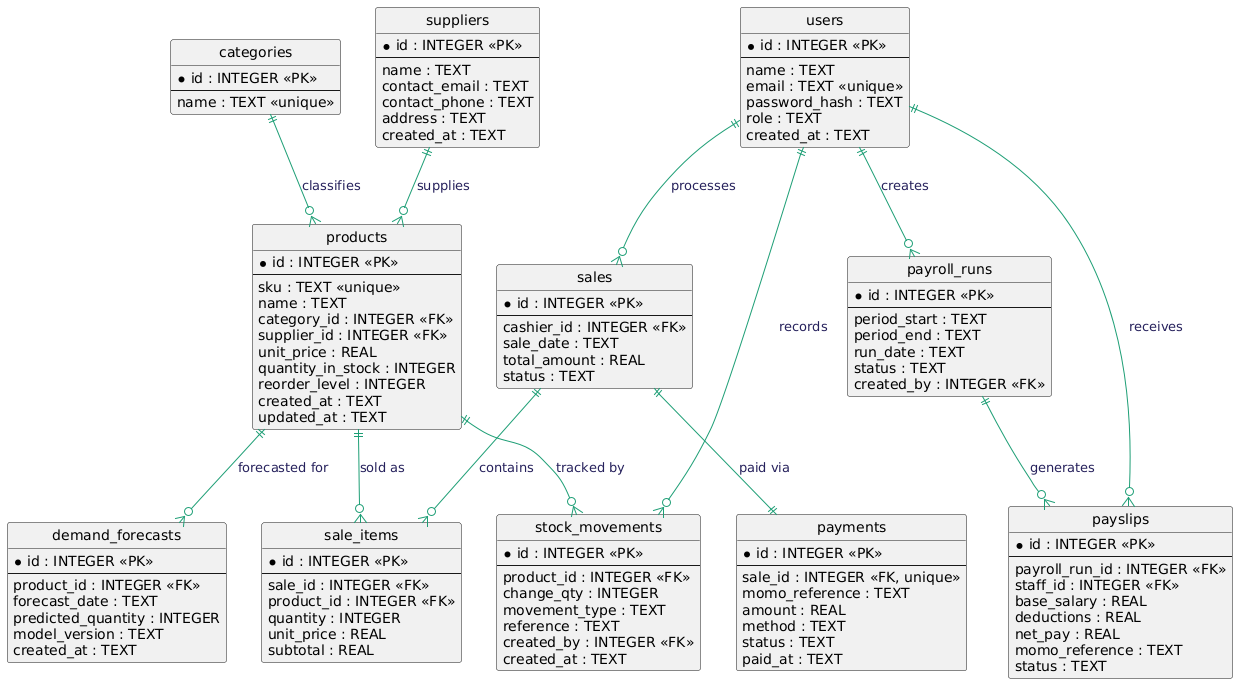
\includegraphics[width=\linewidth]{figures/er_diagram.png}
  \caption{Combined Entity-Relationship Diagram for \sysname{} (Inventory, Sales, Staff \& Payroll)}
  \label{fig:erd}
\end{figure}

\clearpage
\section{Relationship Summary}
\begin{center}
\begin{tabular}{@{}p{3.6cm}p{1.4cm}p{3.6cm}p{5.5cm}@{}}
\toprule
\textbf{From} & \textbf{Card.} & \textbf{To} & \textbf{Meaning} \\
\midrule
categories & 1--N & products & A category classifies many products. \\
suppliers & 1--N & products & A supplier supplies many products. \\
products & 1--N & stock\_movements & A product has many stock movements over time. \\
users & 1--N & stock\_movements & A staff member records many stock movements. \\
users & 1--N & sales & A cashier processes many sales. \\
sales & 1--N & sale\_items & A sale contains many line items. \\
products & 1--N & sale\_items & A product appears in many sale line items. \\
sales & 1--1 & payments & Each sale has exactly one payment record. \\
products & 1--N & demand\_forecasts & A product has many forecast entries over time. \\
users & 1--N & payroll\_runs & An admin creates many payroll runs. \\
payroll\_runs & 1--N & payslips & A payroll run generates many payslips. \\
users & 1--N & payslips & A staff member receives many payslips (one per run). \\
\bottomrule
\end{tabular}
\end{center}

% ================= CHAPTER 3: RELATIONAL SCHEMA =================
\chapter{Relational Schema}

\section{Overview}
Each table below is presented with its columns, data types, and constraints.
The full executable schema is provided as a single SQL file,
\texttt{database/schema.sql}, so this section mirrors that file rather than
duplicating a separate design. All tables are in \textbf{Third Normal Form
(3NF)}: every non-key column depends only on the whole primary key, and no
data that has one true source (e.g. a product's current price) is
duplicated elsewhere as a mutable copy.

\section{Module 1: Inventory}

\subsection*{categories}
\begin{center}
\begin{tabular}{@{}p{3.4cm}p{2.6cm}p{7.5cm}@{}}
\schemahead
id & INTEGER & PRIMARY KEY AUTOINCREMENT \\
name & TEXT & NOT NULL, UNIQUE \\
\bottomrule
\end{tabular}
\end{center}

\subsection*{suppliers}
\begin{center}
\begin{tabular}{@{}p{3.4cm}p{2.6cm}p{7.5cm}@{}}
\schemahead
id & INTEGER & PRIMARY KEY AUTOINCREMENT \\
name & TEXT & NOT NULL \\
contact\_email & TEXT & \\
contact\_phone & TEXT & \\
address & TEXT & \\
created\_at & TEXT & NOT NULL, DEFAULT datetime('now') \\
\bottomrule
\end{tabular}
\end{center}

\subsection*{products}
\begin{center}
\begin{tabular}{@{}p{3.6cm}p{2.6cm}p{7.3cm}@{}}
\schemahead
id & INTEGER & PRIMARY KEY AUTOINCREMENT \\
sku & TEXT & NOT NULL, UNIQUE \\
name & TEXT & NOT NULL \\
category\_id & INTEGER & NOT NULL, FK $\rightarrow$ categories(id) \\
supplier\_id & INTEGER & FK $\rightarrow$ suppliers(id), nullable \\
unit\_price & REAL & NOT NULL, CHECK $\geq 0$ \\
quantity\_in\_stock & INTEGER & NOT NULL, DEFAULT 0, CHECK $\geq 0$ \\
reorder\_level & INTEGER & NOT NULL, DEFAULT 10 \\
created\_at & TEXT & NOT NULL, DEFAULT datetime('now') \\
updated\_at & TEXT & NOT NULL, DEFAULT datetime('now') \\
\bottomrule
\end{tabular}
\end{center}

\subsection*{stock\_movements}
\begin{center}
\begin{tabular}{@{}p{3.6cm}p{2.6cm}p{7.3cm}@{}}
\schemahead
id & INTEGER & PRIMARY KEY AUTOINCREMENT \\
product\_id & INTEGER & NOT NULL, FK $\rightarrow$ products(id) \\
change\_qty & INTEGER & NOT NULL (signed: positive = in, negative = out) \\
movement\_type & TEXT & NOT NULL, CHECK IN ('RECEIPT','SALE','ADJUSTMENT','RETURN') \\
reference & TEXT & e.g. purchase order or sale ID \\
created\_by & INTEGER & FK $\rightarrow$ users(id), nullable \\
created\_at & TEXT & NOT NULL, DEFAULT datetime('now') \\
\bottomrule
\end{tabular}
\end{center}

\section{Module 2: Sales}

\subsection*{sales}
\begin{center}
\begin{tabular}{@{}p{3.6cm}p{2.6cm}p{7.3cm}@{}}
\schemahead
id & INTEGER & PRIMARY KEY AUTOINCREMENT \\
cashier\_id & INTEGER & NOT NULL, FK $\rightarrow$ users(id) \\
sale\_date & TEXT & NOT NULL, DEFAULT datetime('now') \\
total\_amount & REAL & NOT NULL, DEFAULT 0, CHECK $\geq 0$ \\
status & TEXT & NOT NULL, DEFAULT 'pending', CHECK IN ('pending','paid','cancelled') \\
\bottomrule
\end{tabular}
\end{center}

\subsection*{sale\_items}
\begin{center}
\begin{tabular}{@{}p{3.6cm}p{2.6cm}p{7.3cm}@{}}
\schemahead
id & INTEGER & PRIMARY KEY AUTOINCREMENT \\
sale\_id & INTEGER & NOT NULL, FK $\rightarrow$ sales(id) \\
product\_id & INTEGER & NOT NULL, FK $\rightarrow$ products(id) \\
quantity & INTEGER & NOT NULL, CHECK $> 0$ \\
unit\_price & REAL & NOT NULL, CHECK $\geq 0$ (price snapshot at sale time) \\
subtotal & REAL & NOT NULL, CHECK $\geq 0$ \\
\bottomrule
\end{tabular}
\end{center}

\begin{infobox}
\textbf{Why \texttt{unit\_price} is repeated here.} Storing the unit price on
\texttt{sale\_items} is \emph{not} a 3NF violation: it is a historical fact
("this item sold for 500 XAF on this date"), not a duplicate of
\texttt{products.unit\_price}, which can change tomorrow. Removing it would
make past receipts incorrect whenever a price changes.
\end{infobox}

\subsection*{payments}
\begin{center}
\begin{tabular}{@{}p{3.6cm}p{2.6cm}p{7.3cm}@{}}
\schemahead
id & INTEGER & PRIMARY KEY AUTOINCREMENT \\
sale\_id & INTEGER & NOT NULL, UNIQUE, FK $\rightarrow$ sales(id) (1:1) \\
momo\_reference & TEXT & mobile money gateway reference \\
amount & REAL & NOT NULL, CHECK $\geq 0$ \\
method & TEXT & NOT NULL, DEFAULT 'momo', CHECK IN ('momo','cash','card') \\
status & TEXT & NOT NULL, DEFAULT 'pending', CHECK IN ('pending','approved','declined') \\
paid\_at & TEXT & nullable \\
\bottomrule
\end{tabular}
\end{center}

\subsection*{demand\_forecasts}
\begin{center}
\begin{tabular}{@{}p{3.6cm}p{2.6cm}p{7.3cm}@{}}
\schemahead
id & INTEGER & PRIMARY KEY AUTOINCREMENT \\
product\_id & INTEGER & NOT NULL, FK $\rightarrow$ products(id) \\
forecast\_date & TEXT & NOT NULL \\
predicted\_quantity & INTEGER & NOT NULL, CHECK $\geq 0$ \\
model\_version & TEXT & NOT NULL, DEFAULT 'v1' \\
created\_at & TEXT & NOT NULL, DEFAULT datetime('now') \\
\bottomrule
\end{tabular}
\end{center}

\section{Module 3: Staff \& Payroll}

\subsection*{users (shared staff identity)}
\begin{center}
\begin{tabular}{@{}p{3.6cm}p{2.6cm}p{7.3cm}@{}}
\schemahead
id & INTEGER & PRIMARY KEY AUTOINCREMENT \\
name & TEXT & NOT NULL \\
email & TEXT & NOT NULL, UNIQUE \\
password\_hash & TEXT & NOT NULL (bcrypt hash, from Week 1 auth-service) \\
role & TEXT & NOT NULL, CHECK IN ('admin','cashier') \\
created\_at & TEXT & NOT NULL, DEFAULT datetime('now') \\
\bottomrule
\end{tabular}
\end{center}

\subsection*{payroll\_runs}
\begin{center}
\begin{tabular}{@{}p{3.6cm}p{2.6cm}p{7.3cm}@{}}
\schemahead
id & INTEGER & PRIMARY KEY AUTOINCREMENT \\
period\_start & TEXT & NOT NULL \\
period\_end & TEXT & NOT NULL \\
run\_date & TEXT & NOT NULL, DEFAULT datetime('now') \\
status & TEXT & NOT NULL, DEFAULT 'draft', CHECK IN ('draft','processed','paid') \\
created\_by & INTEGER & FK $\rightarrow$ users(id), nullable \\
\bottomrule
\end{tabular}
\end{center}

\subsection*{payslips}
\begin{center}
\begin{tabular}{@{}p{3.6cm}p{2.6cm}p{7.3cm}@{}}
\schemahead
id & INTEGER & PRIMARY KEY AUTOINCREMENT \\
payroll\_run\_id & INTEGER & NOT NULL, FK $\rightarrow$ payroll\_runs(id) \\
staff\_id & INTEGER & NOT NULL, FK $\rightarrow$ users(id) \\
base\_salary & REAL & NOT NULL, CHECK $\geq 0$ \\
deductions & REAL & NOT NULL, DEFAULT 0, CHECK $\geq 0$ \\
net\_pay & REAL & NOT NULL, CHECK $\geq 0$ \\
momo\_reference & TEXT & payout reference \\
status & TEXT & NOT NULL, DEFAULT 'pending', CHECK IN ('pending','paid') \\
\multicolumn{3}{@{}l}{UNIQUE(payroll\_run\_id, staff\_id) -- one payslip per staff member per run} \\
\bottomrule
\end{tabular}
\end{center}

% ================= CHAPTER 4: NORMALIZATION =================
\chapter{Normalization Rationale (3NF)}

\begin{itemize}[leftmargin=1.4em]
  \item \textbf{1NF:} every column holds a single atomic value (e.g. no
  comma-separated lists of product IDs inside a text field).
  \item \textbf{2NF:} every table uses a single-column surrogate primary key
  (\texttt{id}), so there are no partial dependencies on part of a composite
  key.
  \item \textbf{3NF:} non-key columns depend only on the primary key.
  Concretely: a product's category name is not stored on \texttt{products}
  itself, only \texttt{category\_id}, avoiding a transitive dependency
  through \texttt{categories.name}; a payslip's staff name is not duplicated
  from \texttt{users}, only \texttt{staff\_id} is stored.
  \item Two deliberate, justified departures from a naive reading of 3NF
  are documented above: \texttt{sale\_items.unit\_price} (a price
  snapshot, i.e.\ a historical fact) and \texttt{sales.total\_amount} (a
  cached aggregate of \texttt{sale\_items.subtotal}, kept for fast
  reporting and updated in the same transaction as the line items).
\end{itemize}

% ================= CHAPTER 5: INDEXING =================
\chapter{Indexing Strategy}

\section{Indexes Added}
\begin{center}
\begin{tabular}{@{}p{4.6cm}p{4.9cm}p{4.5cm}@{}}
\toprule
\textbf{Index} & \textbf{Table.Column} & \textbf{Query it speeds up} \\
\midrule
idx\_products\_name & products.name & Searching a product by name at checkout \\
idx\_products\_category & products.category\_id & Listing all products in a category \\
idx\_stock\_movements\_product & stock\_movements.product\_id & Stock history for one product \\
idx\_sales\_sale\_date & sales.sale\_date & Sales reports over a date range \\
idx\_sales\_cashier & sales.cashier\_id & A cashier's own sales history \\
idx\_sale\_items\_sale & sale\_items.sale\_id & Line items for a given receipt \\
idx\_demand\_forecasts\_product & demand\_forecasts.product\_id & Forecast history for one product \\
idx\_payslips\_staff & payslips.staff\_id & A staff member's payslip history \\
\bottomrule
\end{tabular}
\end{center}

\begin{infobox}
\textbf{Beyond the minimum.} The exam asks for at least 2 indexes on
frequently-searched tables; the schema adds 8, covering every foreign key
that is likely to be filtered on and the two columns (\texttt{name},
\texttt{sale\_date}) most likely to be searched live during the Week 2
evaluation. \texttt{users.email} and \texttt{products.sku} already get a
free index from their \texttt{UNIQUE} constraints.
\end{infobox}

\section{Proving Index Usage Live}
Run \texttt{database/scripts/explain\_query.sh} to print SQLite's query plan
for two sample queries. A plan line reading
\texttt{SEARCH products USING INDEX idx\_products\_name (name=?)} (rather
than \texttt{SCAN products}) confirms the index was used instead of a full
table scan.

% ================= CHAPTER 6: BACKUP & RESTORE =================
\chapter{Backup and Restore Procedure}

\section{Approach}
SQLite's own \texttt{.backup} command is used rather than a plain file copy,
because it produces a consistent snapshot even if a connection is open, and
\texttt{.restore} reloads it in place. Three scripts under
\texttt{database/scripts/} automate this for the live evaluation:

\begin{enumerate}[leftmargin=1.4em]
  \item \texttt{init\_db.sh} -- creates \texttt{smartstock.db} from
  \texttt{schema.sql} and loads \texttt{seed.sql}.
  \item \texttt{backup\_db.sh} -- writes a timestamped copy to
  \texttt{database/backups/}.
  \item \texttt{restore\_db.sh} -- restores from the most recent backup (or
  one given explicitly) and prints row counts per table as proof.
\end{enumerate}

\section{Demonstration Sequence (used in the evaluation)}
\begin{enumerate}[leftmargin=1.4em]
  \item \texttt{./database/scripts/init\_db.sh} -- fresh database with seed data.
  \item \texttt{./database/scripts/backup\_db.sh} -- creates a backup file.
  \item Delete data on purpose, e.g.\ \texttt{sqlite3 database/smartstock.db "DELETE FROM products;"}
  \item \texttt{./database/scripts/restore\_db.sh} -- restores from the backup.
  \item Confirm row counts are back to their original values (printed
  automatically by the script).
\end{enumerate}

\end{document}